\documentclass{beamer}
% \documentclass[compress]{beamer}

\usetheme{Berlin}
\usecolortheme{beaver}

\newcommand{\itemcolor}{darkred!60!gray}
\setbeamercovered{transparent}
\beamertemplatenavigationsymbolsempty
% \setbeamertemplate{section in toc}[circle]
% \setbeamertemplate{subsection in toc}[circle]
% \setbeamertemplate{itemize items}[circle]
% \setbeamertemplate{enumerate items}[circle]
\setbeamercolor{itemize item}{fg=\itemcolor}
\setbeamercolor{item projected}{bg=\itemcolor}

\AtBeginSection{\frame{\sectionpage}}
% \AtBeginSubsection{\frame{\subsectionpage}}
\AtBeginSubsection[]
{
    \begin{frame}{Outline}
        \tableofcontents[currentsection,currentsubsection]
    \end{frame}
}

% \useoutertheme{infolines}
% \setbeamertemplate{headline}{} % removes the headline that infolines inserts
\newcommand*\oldmacro{}%
\let\oldmacro\insertshorttitle%
\renewcommand*\insertshorttitle{%
   \oldmacro\hfill%
   \insertframenumber\,/\,\inserttotalframenumber}


\usepackage[english]{babel}
\usepackage{caption}
\usepackage{pdfpcnotes}
\usepackage{fontspec}
\usepackage{color}
\usepackage{listings}
\usepackage{lstlinebgrd}
\usepackage{pgf, pgffor}
\usepackage{xkeyval}
\usepackage{todonotes}
\presetkeys{todonotes}{inline}{}
\setsansfont[Ligatures=TeX]{Source Sans Pro}
% \setsansfont{FreeSans}
\setmonofont[Scale=MatchLowercase]{Source Code Pro}
% \setmonofont{DejaVu Sans Mono}
\renewcommand\mathfamilydefault{\rmdefault}

\title{Design and implementation of an \\ Energy-Aware VCPU Scheduler for Linux Kernel}
\date{31. March, 2015} 
\institute{
  Fakult\"at f\"ur Elektrotechnik und Informatik\\
  TU Berlin}

\newcommand{\dummyslide}[1][Dummy slide]{
\frame{\frametitle{#1}
  \todo{Insert a slide here about #1}
}}

\newcommand{\simplesection}[1]{\section{#1}\stepcounter{subsection}}
\newcommand{\fixme}[1]{\textcolor{green}{\textbf{#1}}} 

\lstset{ %
% Basic styles
  basicstyle=\small\ttfamily,
  frame=l,                  
  % title=\lstname,                  
  aboveskip=\medskipamount,
  belowskip=\medskipamount,
% Line numbering
  stepnumber=1,                    
  numbers=left,                    
  numbersep=5pt,                   
% Tabs and spaces
  tabsize=4,
  showtabs=false,                  
  showspaces=false,               
  showstringspaces=false,          
  breakatwhitespace=false,        
  breaklines=false,                 
  % escapeinside={\%*}{*)},        
  extendedchars=true,              
% Colors                      
  numberstyle=\color{gray},
  rulecolor=\color{gray},        
  keywordstyle=\color{blue},       
  stringstyle=\color{brown},   
  commentstyle=\color{green!50!black},   
  backgroundcolor=\color{white}, 
}

\makeatletter
%%%%%%%%%%%%%%%%%%%%%%%%%%%%%%%%%%%%%%%%%%%%%%%%%%%%%%%%%%%%%%%%%%%%%%%%%%%%%%
%
% \btIfInRange{number}{range list}{TRUE}{FALSE}
%
% Test in int number <number> is element of a (comma separated) list of ranges
% (such as: {1,3-5,7,10-12,14}) and processes <TRUE> or <FALSE> respectively

\newcount\bt@rangea
\newcount\bt@rangeb

\newcommand\btIfInRange[2]{%
    \global\let\bt@inrange\@secondoftwo%
    \edef\bt@rangelist{#2}%
    \foreach \range in \bt@rangelist {%
        \afterassignment\bt@getrangeb%
        \bt@rangea=0\range\relax%
        \pgfmathtruncatemacro\result{ ( #1 >= \bt@rangea) && (#1 <= \bt@rangeb) }%
        \ifnum\result=1\relax%
            \breakforeach%
            \global\let\bt@inrange\@firstoftwo%
        \fi%
    }%
    \bt@inrange%
}
\newcommand\bt@getrangeb{%
    \@ifnextchar\relax%
        {\bt@rangeb=\bt@rangea}%
        {\@getrangeb}%
}
\def\@getrangeb-#1\relax{%
    \ifx\relax#1\relax%
        \bt@rangeb=100000%   \maxdimen is too large for pgfmath
    \else%
        \bt@rangeb=#1\relax%
    \fi%
}

%%%%%%%%%%%%%%%%%%%%%%%%%%%%%%%%%%%%%%%%%%%%%%%%%%%%%%%%%%%%%%%%%%%%%%%%%%%%%%
%
% \btLstHL<overlay spec>{range list}
%
% TODO BUG: \btLstHL commands can not yet be accumulated if more than one overlay spec match.
% 
\newcommand<>{\btLstHL}[1]{%
  \only#2{\btIfInRange{\value{lstnumber}}{#1}{\color{orange!30}\def\lst@linebgrdcmd{\color@block}}{\def\lst@linebgrdcmd####1####2####3{}}}%
}%
\makeatother


\begin{document}

\frame{\titlepage} 

\frame{\frametitle{Table of contents}\tableofcontents} 

%%%%%%%%%%%%%%%%%%%%%%%%%%%%%%
% Introduction
%%%%%%%%%%%%%%%%%%%%%%%%%%%%%%
\simplesection{Introduction}

\frame{
	\frametitle{Project scope}

	\begin{itemize}
		\item New scheduler for the Linux kernel
		\item Main purpose of the scheduler is to save power on the server
		\item Mainly used to schedule virtual machines
		\item Specifically, QEMU VMs in our project
	\end{itemize}
}

\frame{
	\frametitle{Project idea}

	\begin{itemize}
		\item CPU is allocated to virtual machine CPUs (VCPUs) in superperiods
		\item Each VCPU has a certain time to run 
		\item Proportionally to its predefined share of the CPU 
		\item If there is any time left in a superperiod, save power
	\end{itemize}
}

\frame{
	\frametitle{How the work is divided}

	Scheduler team:

	\begin{itemize}
		\item Armand Zangue
		\item Tamilselvan Shanmugam
		\item Andrii Berezovskyi
	\end{itemize}

	Power team:

	\begin{itemize}
		\item Lukas Braband
		\item Marat Timergaliev
	\end{itemize}

	Devops team:

	\begin{itemize}
		\item Stephan Bauroth
		\item Andrii Berezovskyi
	\end{itemize}
}

\begin{frame}{Agile \& Scrum}
	\begin{itemize}
		\item It's a progressive approach
		\item We knew about it but never practiced it before
		\item It is a bad tool in the wrong hands {\color{white} of Scrum {\scshape master of disaster}}
		\item In general, it slowed us down until December
	\end{itemize}
\end{frame}


%%%%%%%%%%%%%%%%%%%%%%%%%%%%%%
% Scheduler subsystem
%%%%%%%%%%%%%%%%%%%%%%%%%%%%%%
\section{Scheduler subsystem}

%%%%%%%%%%%%%%%%%%%%%%%%%%%%%%%%%%%%%%%%%%%%%%%%%%%%%%%%%%%
%
% SUBSECTION: Overview of scheduler internals & integration
%
%%%%%%%%%%%%%%%%%%%%%%%%%%%%%%%%%%%%%%%%%%%%%%%%%%%%%%%%%%%
\subsection{Overview of scheduler internals \& integration}
    
\begin{frame}{Linux scheduling overview}    
    \begin{itemize}
        \item Linux has a modular scheduler architecture \pause
        \item Allows different scheduling policies to co-exist \pause
        \item Policies are wrapped up in so-called scheduler classes \pause
        \item Implementing a new scheduling policy for Linux mainly consists of writing a new scheduler class
    \end{itemize}
\end{frame}

\begin{frame}{Linux scheduling overview (2)}    
    \begin{itemize}
        \item There are 2 main scheduling classes \pause
        \item Real-Time scheduling class is responsible for \texttt{SCHED\_FIFO} \& \texttt{SCHED\_RR} policies \pause
        \item Completely Fair Scheduler --- for \texttt{SCHED\_NORMAL} \& \texttt{SCHED\_BATCH} policies \pause
        \item Newly created processes are assigned the normal scheduling policy \pause
        \item All forked subprocesses will inherit it
    \end{itemize}
\end{frame}

% \begin{frame}{Linux scheduling overview (3)}
%     \missingfigure{A picture of VCPU with shares, aligned on a superperiod proportional to their share}
% \end{frame}

\begin{frame}{Superperiod}
    \begin{itemize}
        \item Starts when there is at least one task \pause
        \item Schedules tasks from the \texttt{eligible\_q}
        \item Preempted tasks return to \texttt{waiting\_q}\pause
        \item \textit{Idle} period begins when the \texttt{eligible\_q} is empty
    \end{itemize}
\end{frame}

% \dummyslide[vcpus]

\begin{frame}{Idle period}
    \begin{itemize}
        \item When the \texttt{eligible\_q} is empty, our scheduler ``steals'' the \textit{idle} task
        \item This happens only if the superperiod has extra time left\pause
        \item Idle task is scheduled until the end of superperiod
    \end{itemize}
\end{frame}


\begin{frame}[fragile]{Restart of period}
    \begin{itemize}
        \item When the superperiod is finished, the \texttt{eligible\_q} and \texttt{waiting\_q} are swapped
        \item Precisely speaking, special pointer variables are swapped:
            \begin{lstlisting}[language=C,gobble=12]
            tmp = rq->ospj.ptr_waiting_q;
            rq->ospj.ptr_waiting_q = rq->ospj.ptr_eligible_q;
            rq->ospj.ptr_eligible_q = tmp;
            \end{lstlisting} 
        \item Time is then replenished by \texttt{replenish\_super\_period()}
    \end{itemize}
\end{frame}

\begin{frame}{Integrating a scheduler}

{
    With kernel:
    \begin{enumerate}
        \item Struct declarations
        \item Config flags
        \item Scheduler list
    \end{enumerate}
}\pause 

{
    With userspace:
    \begin{enumerate}
        \item Syscall
        \item Userspace tool
    \end{enumerate}
}\pause

{
    With power-saving code:
    \begin{enumerate}
         \item Changing the \texttt{sched\_class} of idle task
         \item Calling the power-related code inside \texttt{idle.c}
    \end{enumerate}
}
\end{frame}

%%%%%%%%%%%%%%%%%%%%%%%%%%%%%%%%%%%%%%%%%%%%%%%%%%%%%%%%%%%
%
% SUBSECTION: Integration with kernel
%
%%%%%%%%%%%%%%%%%%%%%%%%%%%%%%%%%%%%%%%%%%%%%%%%%%%%%%%%%%%
\subsection{Integration with kernel}

\begin{frame}{Custom runqueue}
    \begin{itemize}
        \item Each scheduling class has its runqueue structure \pause
        \item Main runqueue has a field for each scheduling class \pause
        \item The is one (main) runqueue per CPU
    \end{itemize}
\end{frame}

% TODO firstnumber 365
\begin{frame}[fragile]{Custom runqueue: \texttt{struct ospj\_rq}}
\begin{lstlisting}[
language=C,
gobble=0,
linebackgroundcolor={%
    \btLstHL<1>{5,6}%   two queues
    \btLstHL<2>{3,4}%   their pointers
    \btLstHL<3>{7}%     pointer backwards
    \btLstHL<4>{8}%     stealing the idle
    \btLstHL<5>{10}%    stealing request
    \btLstHL<6>{11}%    ticks left in the superperiod
}]
struct ospj_rq {
    struct list_head ospj_list_head;
    struct list_head *ptr_eligible_q;
    struct list_head *ptr_waiting_q;
    struct list_head eligible_q;
    struct list_head waiting_q;
    struct rq *rq;
    struct task_struct *idle;
    unsigned int nr_running;
    unsigned int idle_request;
    unsigned int period_ticks;
};
\end{lstlisting}
\end{frame}

\begin{frame}[fragile]{Main runqueue: \texttt{struct rq}}
\begin{lstlisting}[
language=C,
basicstyle=\small\ttfamily,
gobble=0,
firstnumber=417,
linebackgroundcolor={%
    \btLstHL<1>{422}%
    \btLstHL<2>{421}%
}]
struct rq {
    ...
    struct cfs_rq cfs;
    struct rt_rq rt;
#ifdef CONFIG_SCHED_VMS
    struct ospj_rq ospj;
#endif /* CONFIG_SCHED_VMS */
    ...
}
\end{lstlisting}
\end{frame}


\begin{frame}[fragile]{Task structure}
\pnote{Each task in the system is assigned to a particular scheduling class}
\begin{lstlisting}[
language=C,
basicstyle=\small\ttfamily,
% basicstyle=\footnotesize\ttfamily,
gobble=0,
firstnumber=1055,
linebackgroundcolor={%
    \btLstHL<1>{1065,1057}%
    \btLstHL<2>{1060,1062}%
    \btLstHL<3>{1061}%
}]
struct task_struct {
    ...
    const struct sched_class *sched_class;
    ...
#ifdef CONFIG_SCHED_VMS
    unsigned int share;
    unsigned int ospj_time_slice;
    unsigned int ospj_assigned_time_slice;
#endif /* CONFIG_SCHED_VMS */
    ...
    unsigned int policy;
    ...
}
\end{lstlisting}
\end{frame}

\begin{frame}{Configuration options}
    \begin{itemize}
        \item All this code must be integrated into kernel
        \item The integration must be seamless
        \item We used the configuration option declared in \texttt{Kconfig}
    \end{itemize}
\end{frame}

\begin{frame}[fragile]{Configuration options (2)}
    \begin{lstlisting}[language=C,
    gobble=4,
    language=ruby,
    firstnumber=2334,
    linebackgroundcolor={%
        \btLstHL<1>{2334,2340}%
        \btLstHL<2>{2337}%
        \btLstHL<3>{2338}%
        \btLstHL<4>{2336}%
    }
]
    menu "VMS scheduler (OSPJ)"
    
    config SCHED_VMS
        bool "Virtual Machines Scheduling (VMS) policy"
        default y

    endmenu
    \end{lstlisting}
\end{frame}

\begin{frame}{Configuration options (3)}
    \begin{figure}
       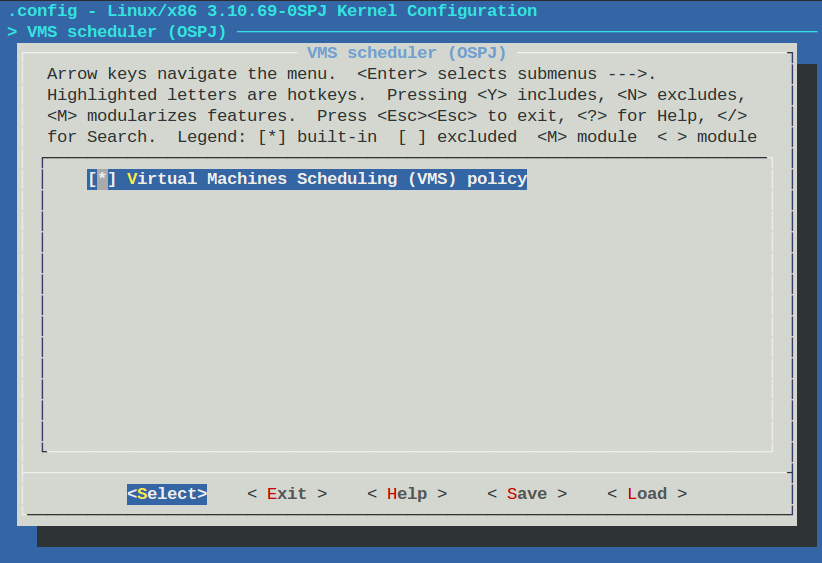
\includegraphics[width=0.8\linewidth]{img/menuconfig.png}
    \end{figure}
\end{frame}


%%%%%%%%%%%%%%%%%%%%%%%%%%%%%%%%%%%%%%%%%%%%%%%%%%%%%%%%%%%
%
% SUBSECTION: Integration with userspace
%
%%%%%%%%%%%%%%%%%%%%%%%%%%%%%%%%%%%%%%%%%%%%%%%%%%%%%%%%%%%

\subsection{Integration with userspace}

\begin{frame}{\texttt{sched\_setscheduler(2)} syscall}
    \begin{itemize}
        \item Used to set the scheduler and priority
        \item Validates parameters before making changes
        \item We extended it to handle \texttt{SCHED\_VMS} policy
        \item And accept the \texttt{share} parameter
    \end{itemize}
\end{frame}

\begin{frame}[fragile]{\texttt{struct sched\_param}}
\begin{lstlisting}[language=C,linebackgroundcolor={%
        \btLstHL<1>{4}%
    }]
struct sched_param {
    int sched_priority;
#ifdef CONFIG_SCHED_VMS
    unsigned int share;
#endif /* CONFIG_SCHED_VMS */
};
\end{lstlisting}
\end{frame}

\begin{frame}{Userspace headers}
    \begin{itemize}
        \item Required by the userspace tools at the compilation phase
        \item Must match the installed kernel
        \item Automatically installed on \texttt{deneb} with DevOps help on each build
        \item Main file changes to \texttt{/usr/include/linux/sched.h}
    \end{itemize}
\end{frame}

\begin{frame}[fragile]{Userspace headers (2)}

Typical use case:

\begin{lstlisting}[language=C]
#ifdef SCHED_VMS
    vms_support = "ENABLED";
#else
    vms_support = "DISABLED";
#endif
\end{lstlisting}
\end{frame}

\begin{frame}{All together: {\ttfamily\bfseries ospj-setsched} tool}
    \begin{itemize}
        \item Designed to \textbf{change} and \textbf{retrieve} the scheduling policies
        \item Allows to set the {\bfseries {\ttfamily SCHED\_VMS}} policy
        \item Allows to supply the {\bfseries task {\itshape share}} (for OSPJ scheduler)
    \end{itemize}
\end{frame}

\begin{frame}{Changing policy for QEMU threads}
    \begin{itemize}
        \item Is main design target of the \texttt{ospj-setsched} tool
        \item Minimally, only change the policy for the threads corresponding to the VCPUs
        \item Also, possible to schedule other threads:
        \begin{itemize}
            \item Configuration dependent threads
            \item Worker threads
            \item Dedicated threads
            \item Reusable threads 
        \end{itemize}
    \end{itemize}
\end{frame}


\subsection{Evaluation}

\begin{frame}{Scheduler fairness measurement}
    \begin{enumerate}
        \item Calculate $N$th element of the Fibonacci series
        \item Time it inside QEMU
        \item \texttt{time fibo 10,000,000 > /dev/null}
    \end{enumerate}
\end{frame}

\begin{frame}{Scheduler fairness measurement results}
    \begin{figure}
       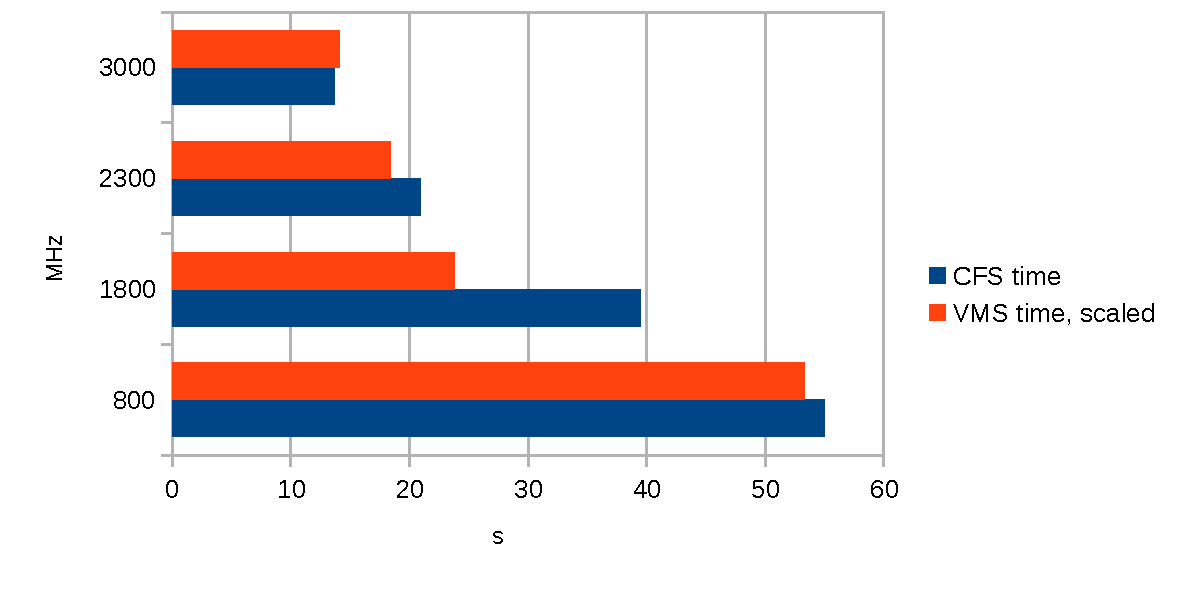
\includegraphics[width=1\linewidth]{img/fibo.pdf}
    \end{figure}
\end{frame}


%%%%%%%%%%%%%%%%%%%%%%%%%%%%%%
% Power-saving subsystem
%%%%%%%%%%%%%%%%%%%%%%%%%%%%%%
\simplesection{Power-saving subsystem}
\lstset{
	language=C,
	basicstyle=\tiny,
	numbers=none,
	frame=none,
	tabsize=4,
	showtabs=false
}
	

\subsection{Power Management}
    
\frame{
    \frametitle{Power management approaches}
    \begin{itemize}
        \item Sleeping states (C-States)
        \item Core disabling.
        \item Dynamic frequency scaling (P-states)
    \end{itemize}
}

\frame{
    \frametitle{Speeping states \& C-States}
    \begin{itemize}
        \item What is a C-state?
        \item Requirements
        \item How to enable?  
        \item Fail and hunt for an approach
    \end{itemize}
}



\frame {
    \frametitle{Sleeping states. What is a C-state?}
    \begin{itemize}
        \item Definition
        \item The basic power states: C0, C1, C2, C3
        \item Architecture specific difference
    \end{itemize}
}

\frame {
    \frametitle{Sleeping states. Requirements}
    \begin{itemize}
        \item BIOS ACPI component
        \item ACPI module
        \item CPU idle driver
    \end{itemize}
}

\begin{frame}[fragile]
{ACPI module installation configuration}
\begin{lstlisting}[language=C,gobble=0]
CONFIG_PM=y
CONFIG_ACPI=y
CONFIG_ACPI_AC=y
CONFIG_ACPI_BATTERY=y
CONFIG_ACPI_BUTTON=y
CONFIG_ACPI_FAN=y
CONFIG_ACPI_PROCESSOR=y
CONFIG_ACPI_THERMAL=y
CONFIG_ACPI_BLACKLIRG_YEAR=0
CONFIG_ACPI_EC=y
CONFIG_ACPI_POWER=y
CONFIG_ACPI_SYSTEM=y
\end{lstlisting}
\end{frame}


\begin{frame}[fragile]
	{Sleeping states. How to enable C1?}
	\begin{itemize}
		\item	Meet the mentioned requirements
		\item	Read specific msr register - {\color{red}MSRC001\_0073}            
		\item[]	\begin{lstlisting}
/*
 * Reading the msr register.
 * @param msr_id - MSR Register to read
 * @return msr_value - The status of reading the register
 */
static long rdmsr_v(long msr_id){		
    long long msr_value;
    asm volatile ( "rdmsr" : "=A" (msr_value) : "c" (msr_id) );
    return msr_value;		
}
\end{lstlisting}
		\item	Or Execute {\color{red}HLT} instruction
	\end{itemize}
\end{frame}


\begin{frame}[fragile]{Fail and hunt for an approach}
	\begin{itemize}
		\item No ACPI configuration in BIOS even with the latest update
		\item Powertop didn't detect available C-states
		\item Specific CPU idle driver absent for our CPU
		\item Approach fail, and hunting green piece energy mode
	\end{itemize}
\end{frame}

\begin{frame}[fragile]{Core disabling}
	\begin{enumerate}
		\item Advantages of the approach. 
		\item[] \lstinline$sudo sh -c 'echo 0 > /sys/devices/system/cpu/cpu1/online'$
		\item Benchmark
	\end{enumerate}
\end{frame}

\frame{
    \frametitle{Benchmark Core disabling vs DFS}
    \begin{table}[h]
        \begin{tabular}{ | l | c | c | c | c|}
    \hline
        Experiments & Cores & Freq      & Energy    & Response          \\ 
        \hline
        1 Baseline  & 4     & 3 GHz     & 77194 Ws  & 0                 \\ 
        \hline
        2           & 3     & 3 GHz     & 71693 Ws  & 15-45ms           \\
        \hline
        3           & 4     & 3 cores on& 73150 Ws  & 5μs               \\
        &       & 3 GHz and &           &                   \\
        &       & 1 core on &           &                   \\
        &       & 800 MHz   &           &                   \\
        \hline
        4           & 4     & 800 MHz   & 37966 Ws  & 5μs               \\
        \hline
        \end{tabular}
    \caption*{All experiments were performed with a cpu-load of 100\%}
    \end{table}
}


\begin{frame}{P-states}
    \begin{enumerate}
        \item With P-states, frequencies can be changed
        \item ACPI-cpufreq allows P-States of AMD Phenom(tm) II X4 940 Processor:
    \end{enumerate}
        \begin{table}[h]
        \begin{tabular}{ | l | c | c |}
    \hline
    P-state & Frequency \\
    \hline
    P0 & 3.0Ghz \\
    P1 & 2.3Ghz \\
    P2 & 1.8Ghz \\
    P3 & 800Mhz \\
    \hline
     \end{tabular}
    \end{table}
\end{frame}

\begin{frame}[fragile]{Ways to switch P-states}
	\begin{itemize}
		\item	Via shell:\\
			\lstinline$cpupower -c 0 frequency-set -f 800000$
		\item	Via shell with sysfs:
			\begin{lstlisting}
sudo sh -c 'echo userspace >
    /sys/devices/system/cpu/cpu0/cpufreq/scaling_governor'
sudo sh -c 'echo 800000 >
    /sys/devices/system/cpu/cpu0/cpufreq/scaling_setspeed'
\end{lstlisting}
		\item	Via c-function:
			\begin{enumerate} 
				\item from \textbf{user}-space with sysfs:\\
					\lstinline$sysfs_set_frequency(unsigned int cpu, unsigned long target_frequency);$
				\item from \textbf{kernel}-space
			\end{enumerate}
	\end{itemize}
\end{frame}

\begin{frame}{P-state-switching from kernel-space}
	\begin{itemize}
		\item interface not clearly defined (yet?) %Comment: under development, mention big load of messages in linux-pm developer-mailing-list
		\item cpufreq\_policy (struct defined in include/linux/cpufreq.h)
		\item Tried to get current policy, manipulate and set it again\\
			$\rightarrow$ But failed
	\end{itemize}
\end{frame}

\begin{frame}[fragile]{Code example P-states}
	\begin{lstlisting}
struct cpufreq_policy *policy, *policy_max, *policy_min;
struct cpufreq_policy *cpu_policy = NULL;
int tmpGetPolicyResult;
int error;
policy = (struct cpufreq_policy*) kmalloc(sizeof (struct cpufreq_policy), GFP_ATOMIC);
policy_max = (struct cpufreq_policy*) kmalloc(sizeof (struct cpufreq_policy), GFP_ATOMIC);
policy_min = (struct cpufreq_policy*) kmalloc(sizeof (struct cpufreq_policy), GFP_ATOMIC);
if (!(policy && policy_max && policy_min))
    /* error handling */
error = cpufreq_get_policy(policy, cpuNo); 
if (!error && policy)
    /* error handling */
memcpy((void*)policy_min, (void*)policy, sizeof(struct cpufreq_policy));
memcpy((void*)policy_max, (void*)policy, sizeof(struct cpufreq_policy));
policy_max->min = 3000000;
policy_max->max = 3000000;
policy_min->min =  800000;
policy_min->max =  800000;
cpufreq_cpu_put(policy_max);
kfree(policy);
policy = NULL;
kfree(policy_min);
policy_min = NULL;
kfree(policy_max);
policy_max = NULL;
\end{lstlisting}
\end{frame}

\begin{frame}{Plan for P-state-switching from kernel-space}
    \begin{itemize}
		\item a governor has a function-pointer store\_setspeed:
		\item \lstinline$int (*store_setspeed) (struct cpufreq policy *policy, unsigned int freq);$
		\item hand over our policy and frequency
		\item fields for min-, max- and cur frequency
    \end{itemize}
\end{frame}


%%%%%%%%%%%%%%%%%%%%%%%%%%%%%%
% Live demo
%%%%%%%%%%%%%%%%%%%%%%%%%%%%%%
\simplesection{Live demo}

%%%%%%%%%%%%%%%%%%%%%%%%%%%%%%
% Devops
%%%%%%%%%%%%%%%%%%%%%%%%%%%%%%
\simplesection{Devops}

\begin{frame}{Git}    
    \begin{itemize}
        \item Git was used for version control during the complete Development
        \item GitLab at TU Berlin was used to host the repository as well as the bug tracker (\texttt{issues} on GitLab)
        \item Branching model was exhausted for automation of the build process by introducing a \texttt{deploy} branch which is queried periodically by \texttt{deneb}
        \item Development of different features or sub projects (scheduler, measurements, power saving, ...) was split across branches
    \end{itemize}
\end{frame}

\begin{frame}{GitLab}
	\begin{itemize}
		\item GitLab is a repository manager including an issue tracker and a wiki
		\item TU Berlin hosts a GitLab server with free, private projects for students
		\item GitLab offers \texttt{hooks} we use to trigger builds in Jenkins and kernel updates on \texttt{deneb}
		\item GitLabs \texttt{issues} have the advantage of being controllable via commit messages and hence were the better choice than redmine tickets
	\end{itemize}
\end{frame}

\begin{frame}{Jenkins}
	\begin{itemize}
		\item \textit{Jenkins CI} is an open source Continuous Integration Framework we used to automatically build the kernel
		\item runs on \texttt{zambezi}, a host within the local network
		\item each commit to the \texttt{master} branch of our repository triggers a compilation
		\item if compilation is successful, the current state of \texttt{master} branch is pushed to \texttt{deploy} branch
		\item successful and failing compilations trigger messages to our group chat
	\end{itemize}
\end{frame}

\begin{frame}{Polling on deneb}
	\begin{itemize}
		\item a cronjob on \texttt{deneb} is checking the \texttt{deploy} branch every 5 minutes for new versions
		\item if a newer version is found, it is pulled, compiled and installed
		\item logging is done to our group chat to alert on unforeseen behaviour
		\item new kernel is fed into \textit{GRUB} to be booted
	\end{itemize}
\end{frame}

\begin{frame}{GRUB on deneb}
	\begin{itemize}
		\item \textit{GRUB} on \texttt{deneb} is configured to once try to boot the newest kernel after its installation
		\item if kernel boot fails, \texttt{deneb} reboots with the second newest kernel available
		\item if booting succeeds, the newest kernel is chosen as default
		\item in all cases, logging to our group chat is ensured
		\item for debugging non-bootable kernels, we installed a serial line to \texttt{zambezi}
	\end{itemize}
\end{frame}

\begin{frame}
	\begin{figure}[h]
		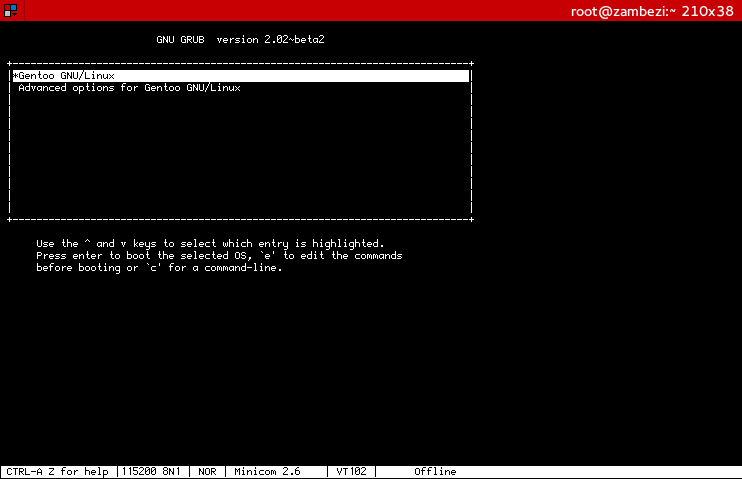
\includegraphics[width=.8\textwidth]{img/serialGRUB.png}
		\caption{GRUB boot choices over minicom on \texttt{zambezi}}
		\label{fig:serialGRUB}
	\end{figure}
\end{frame}

\begin{frame}{QEMU I}
	\begin{itemize}
		\item to test if kernels boot before pushing them to master, an easy-to-use script spawning a QEMU VM was written
		\item central problem was there needs to be a rootfs along with the kernel image for QEMU to be able to boot the kernel
		\item busybox and some base files were crafted together to form a rootfs, whole build is scripted
	\end{itemize}
\end{frame}

\begin{frame}{QEMU II}
	\begin{itemize}
		\item boot-testing opened up the possibility to include userspace tools in the initramfs and hence QEMU was used to debug them too
		\item this setup is also used to simulate the VM that are to be scheduled on \texttt{deneb}
		\item for future work, if one would configure QEMU to emulate a specific processor, the power sub system coud be debugged in QEMU too
		\item \texttt{deneb} would just be needed for measurements
	\end{itemize}
\end{frame}


\end{document}
